\chapter{Stock Price Prediction Analysis}

\section{Introduction}
Stock market prediction is a challenging task due to its uncertanity .In this chapter we will see three diffrent models : long short term memory (LSTM).Random Forest (RF) and sonal AutoRegressive Integrated Moving Average (SARIMA) to predict closing prices .

\section{Dataset Overview}
The dataset chosen for forecasting consists of historical stock market data for investment the company AABA (altaba.inc) 2018.this dataset contains stock transaction data that was recorded everyday from january 3 2006 to january 1 2018.this dataset is very good for time series forecasting as it contains everyday fluctuations in prices .The closing price which is our target variable is very important features because it helps in forecasting future values.

\section{Models used for training}

\subsection{LSTM Model}
Lstm is a type of RNN (Recurrent Neural Network ) designed to handle sequential data .It captures long and short term depndencies and patterns in stock price movements.

\subsection{Training process}
The model was trained to predict closing stock prices from past prices. Following is the training process:- 
    \begin{itemize}
        \item \textbf{Data preparation}:- The closing price fluctuates so the price diffrences of closing price was computed to transform it into stationary series.Lag features were created to predict the following day's price based on previous 5 days.
        \item \textbf{Data Scalling}:- standard scalar was used to normalize the features.
        \item \textbf{Model Architecture}:- The LSTM model was built using these following layers:-
        \begin{itemize}
            \item Input Layer accepts iput sequence.
            \item Lstm Layer
            \item Leaky Relu was used as activation function to prevent dead neurons because they do not contibute in learning
            \item Output Layer generate a predictive value 
        \end{itemize}
    \end{itemize}

\subsection{Random Forest Model}
random Forest is an ensemble learning method that utilizes numerous decision trees to enhance prediction accuracy. It doesnt overfit very easily and works well on structured data .

\subsection{SARIMA Model}
SARIMA, or Seasonal AutoRegressive Integrated Moving Average, is a time-series forecasting model that considers seasonality, trends, and cyclic patterns in data.

\section{Model evaluation}

\subsection{Actual vs Predicted Closing Prices}
In figures Figures \ref{fig:lstm}, \ref{fig:rf}, and \ref{fig:sarima} comaring actual vs predicted closing price diffrences for Lstm,rf and sarima models 
\begin{figure}[H]
    \centering
    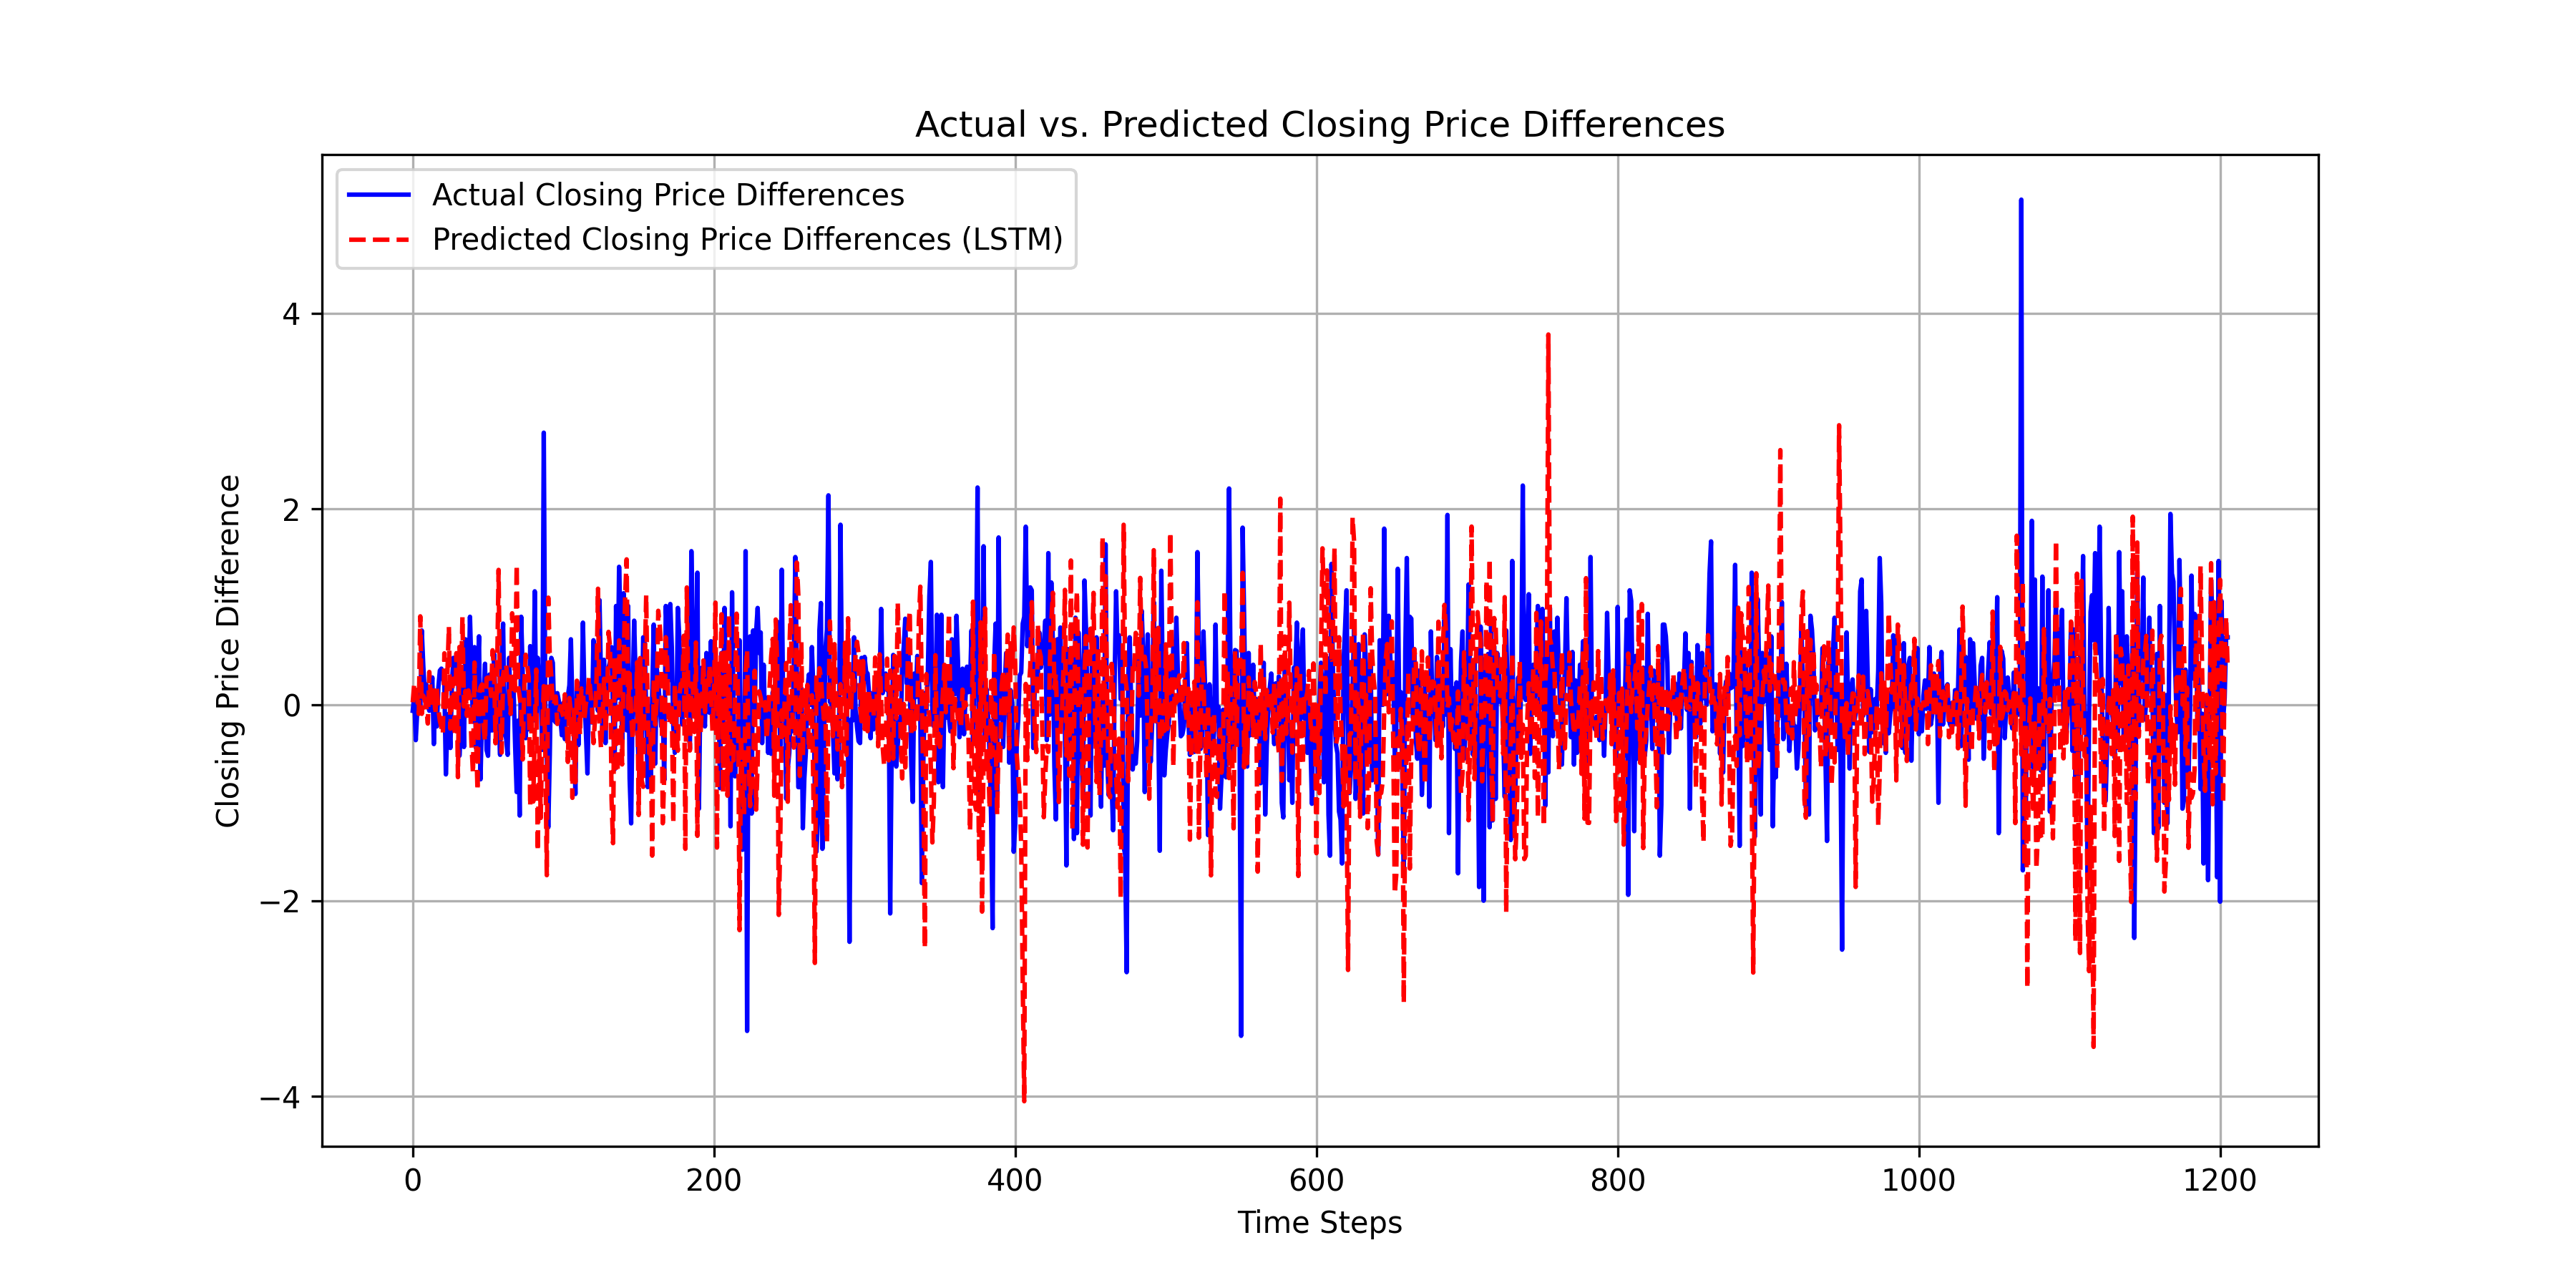
\includegraphics[width=0.8\textwidth]{actual_vs_predicted.png}
    \caption{Actual vs Predicted Closing Price Differences - LSTM}
    \label{fig:lstm}
\end{figure}

\begin{figure}[H]
    \centering
    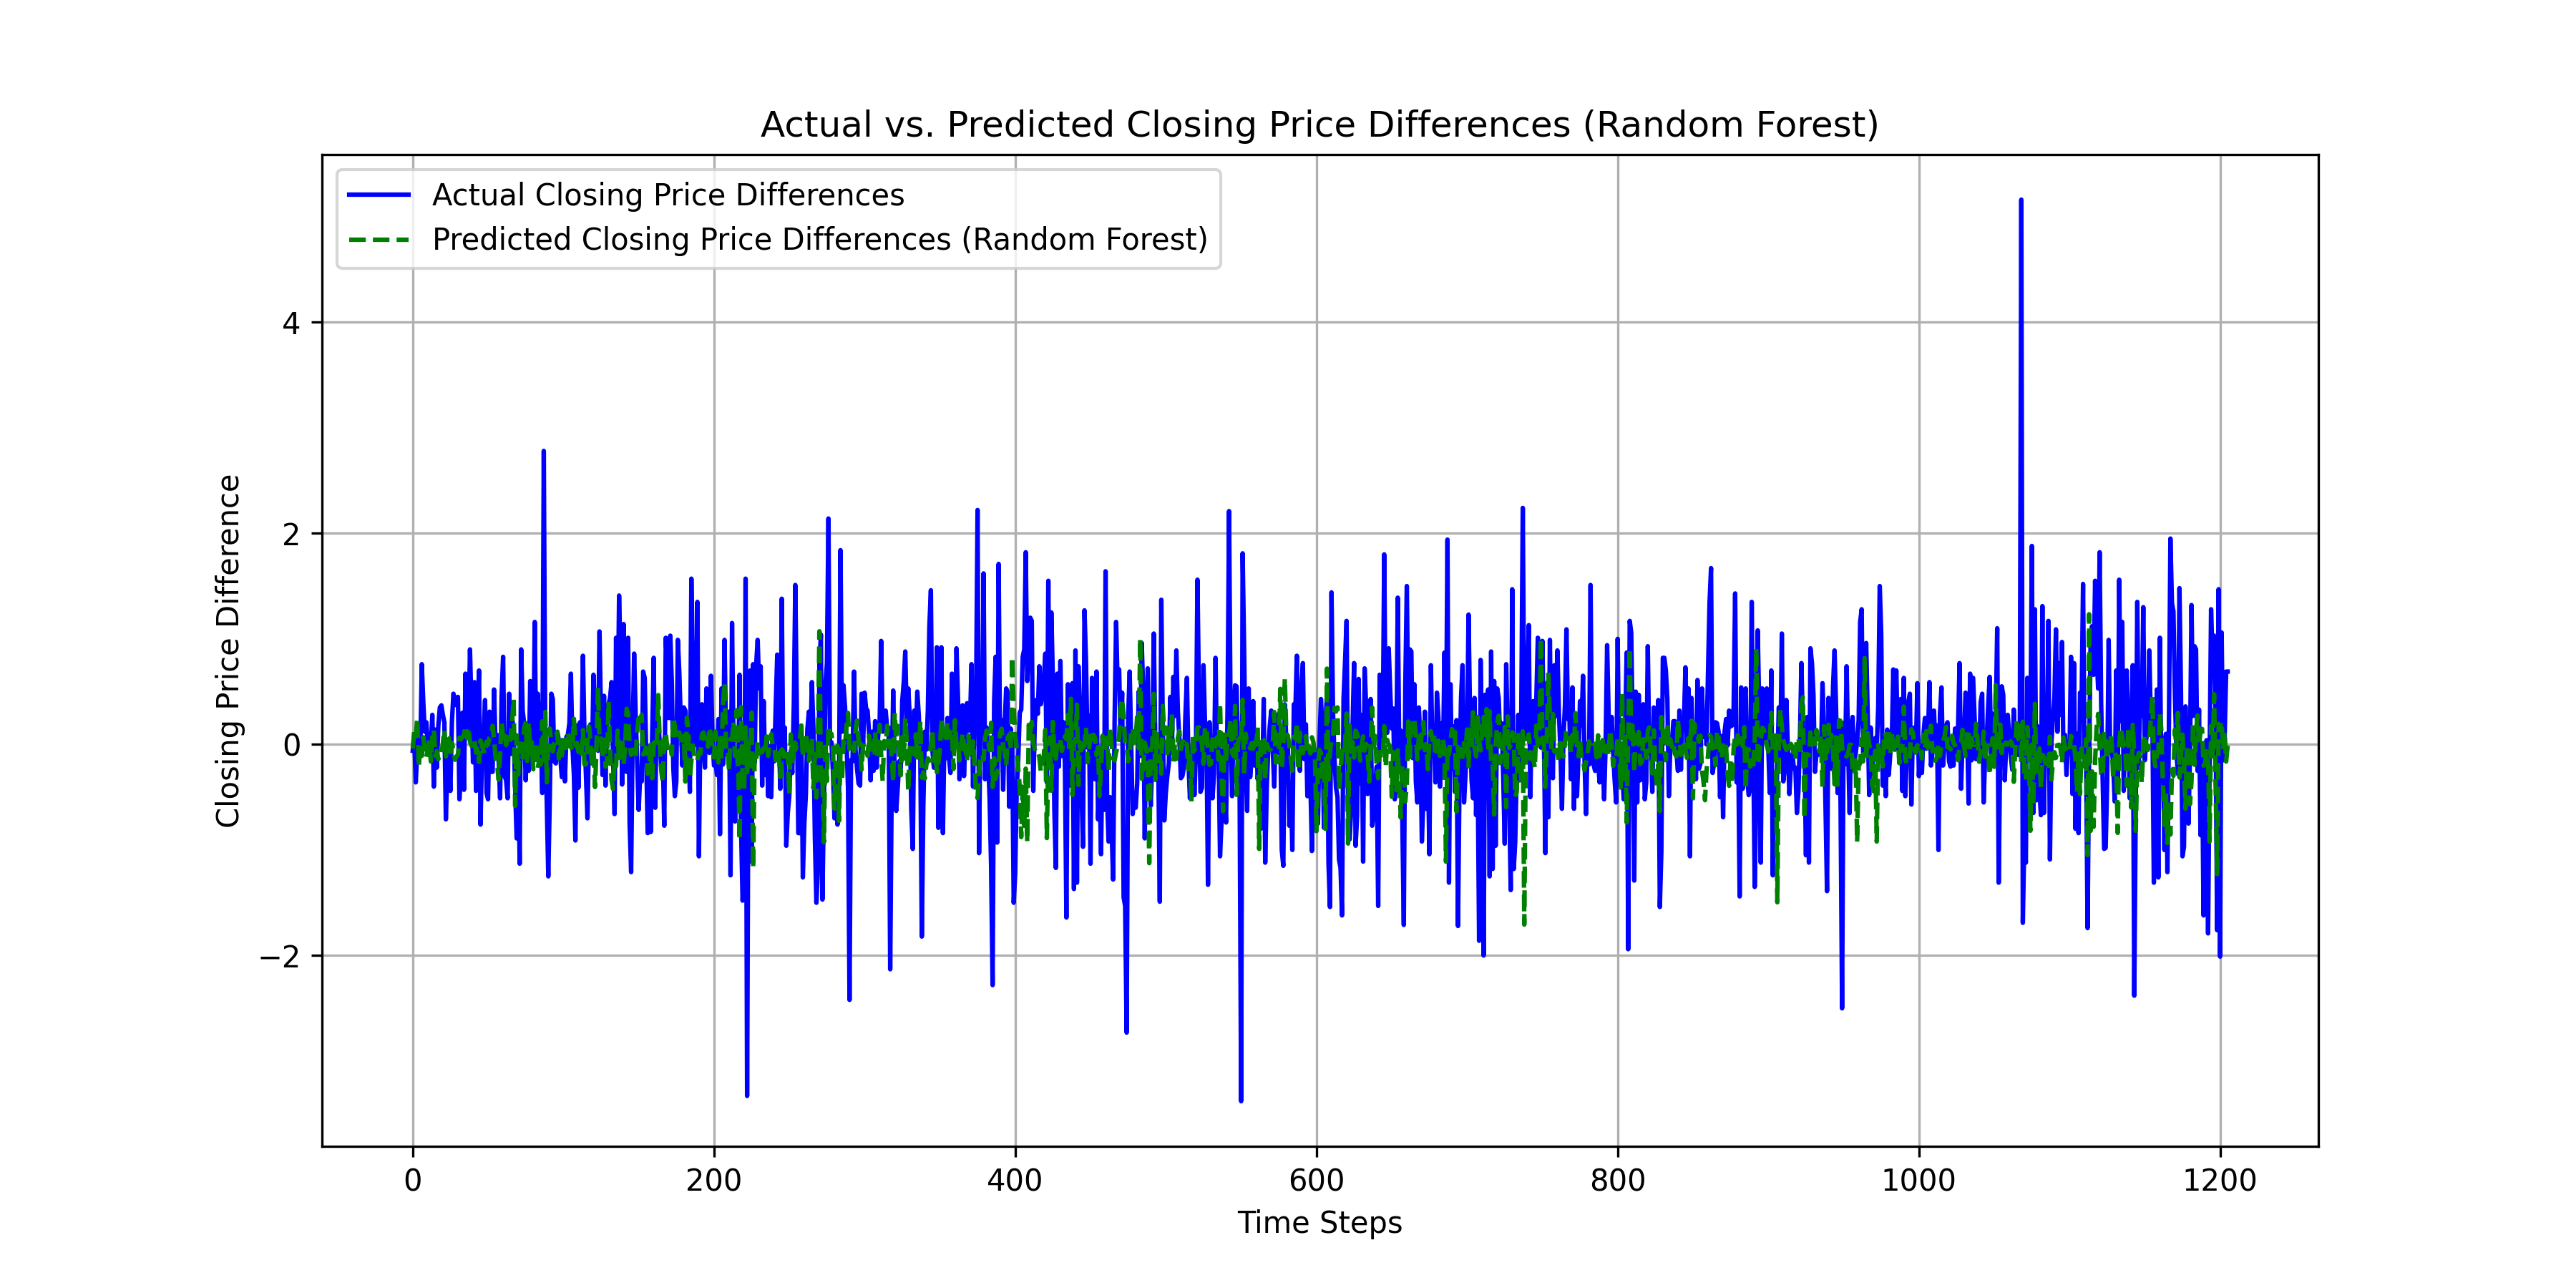
\includegraphics[width=0.8\textwidth]{actual_vs_predicted_rf.png}
    \caption{Actual vs Predicted Closing Price Differences - Random Forest}
    \label{fig:rf}
\end{figure}

\begin{figure}[H]
    \centering
    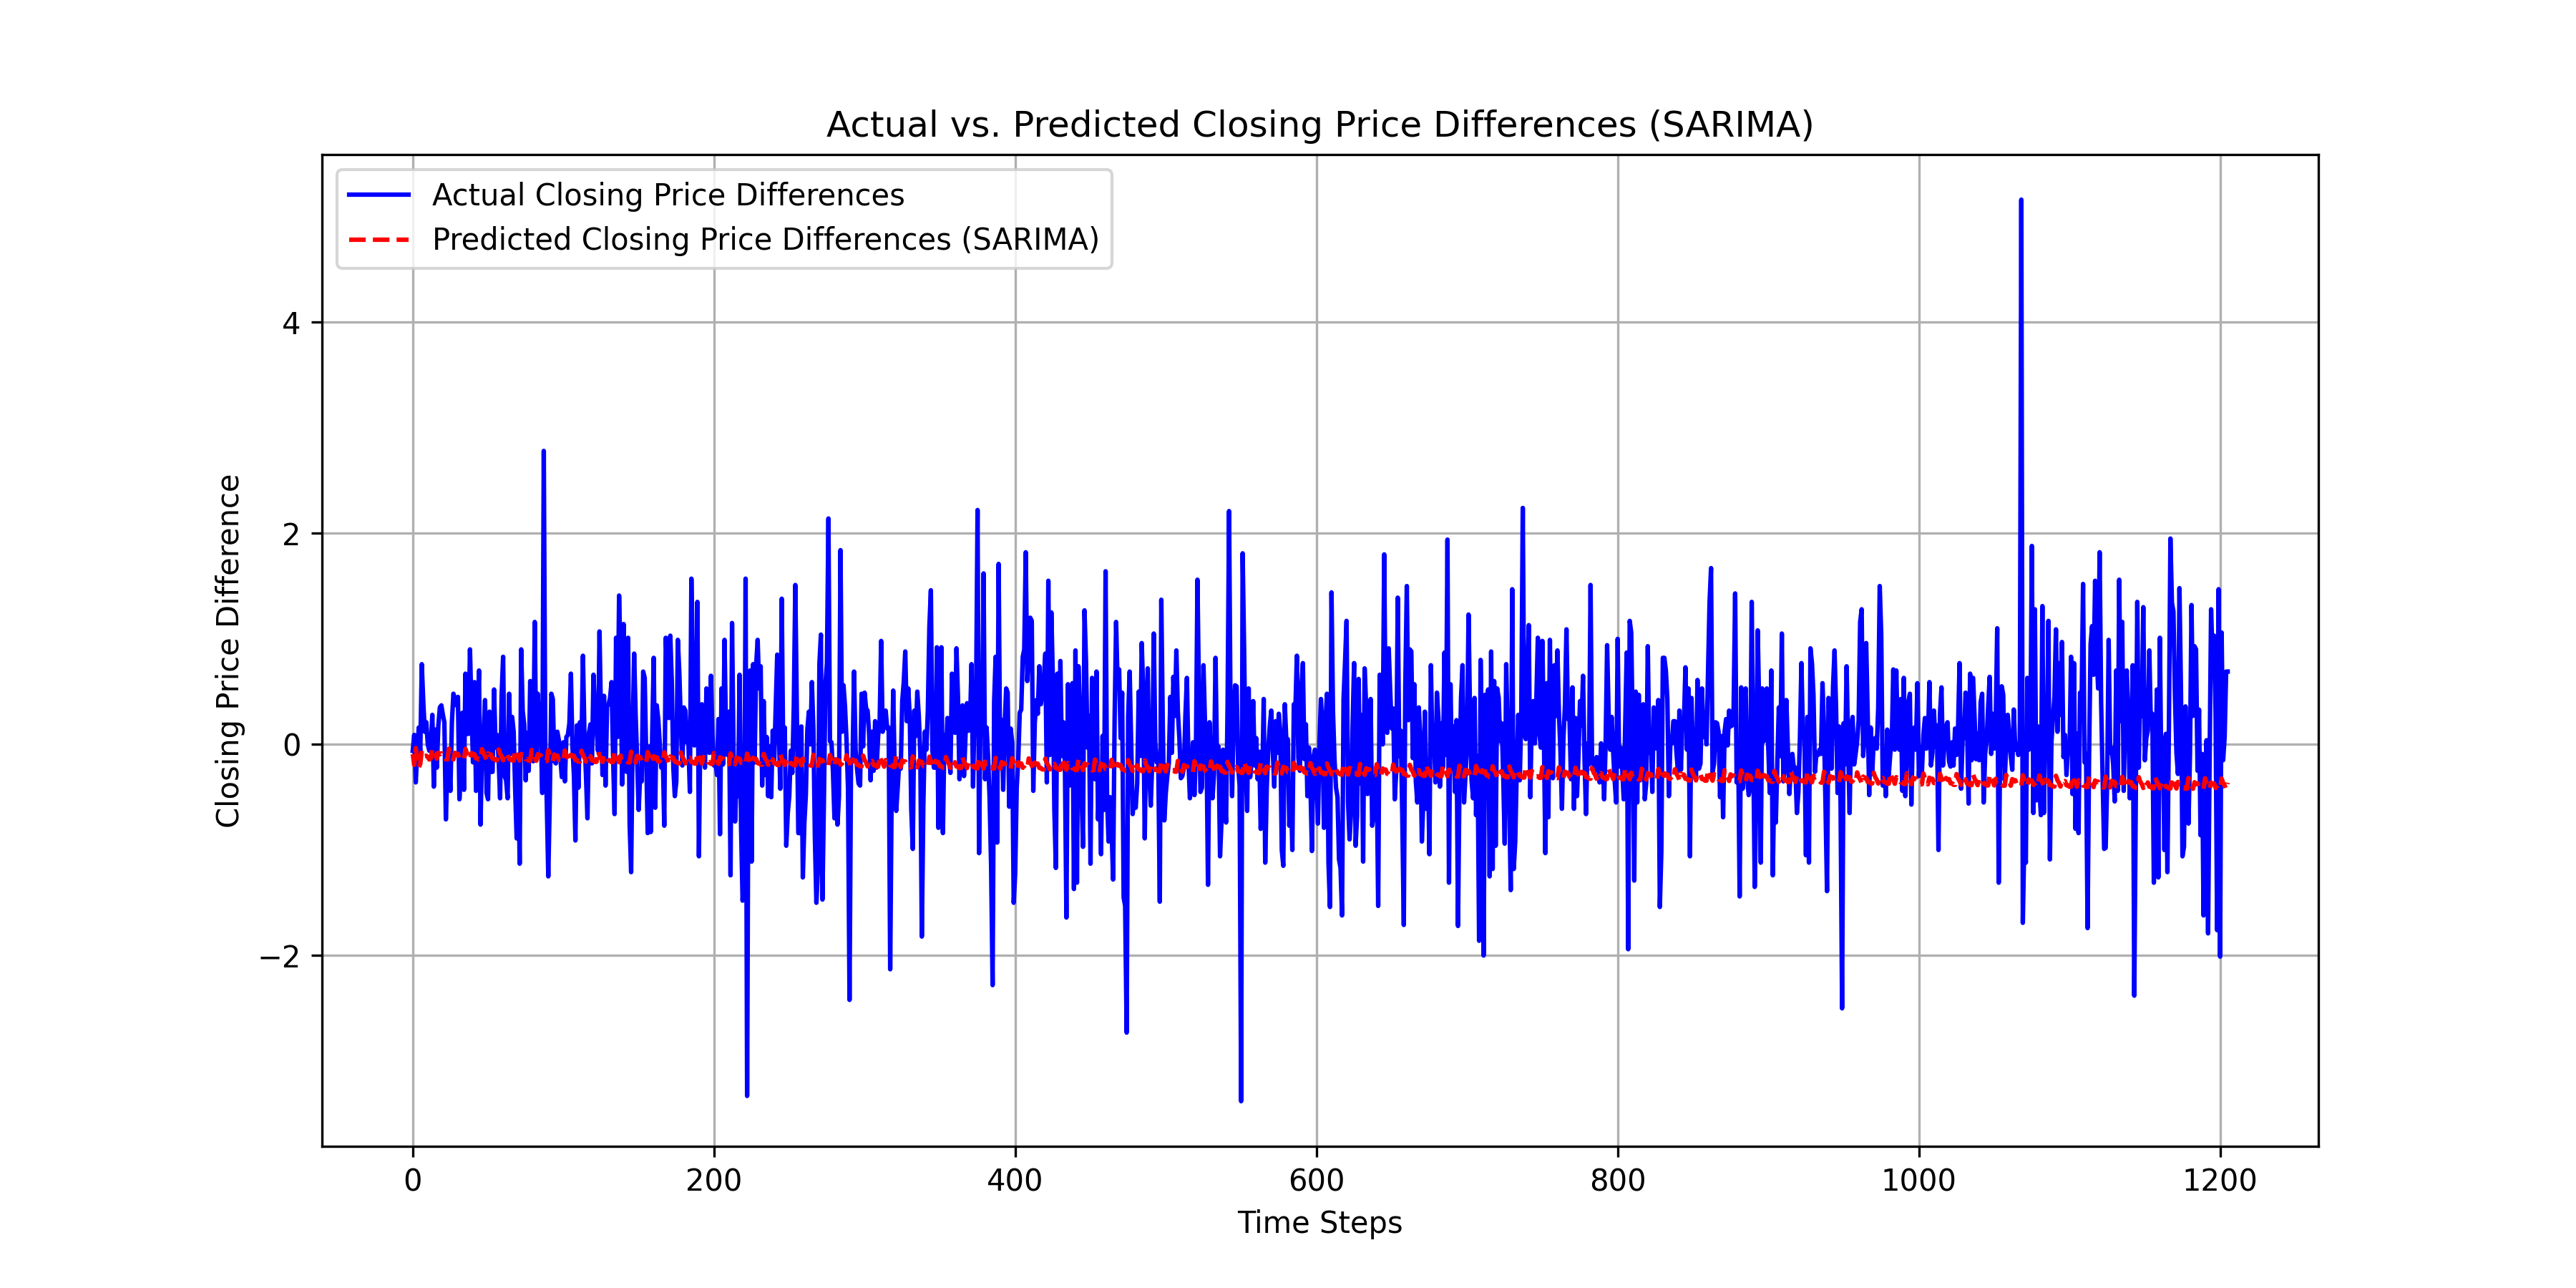
\includegraphics[width=0.8\textwidth]{actual_vs_predicted_sarima.png}
    \caption{Actual vs Predicted Closing Price Differences - SARIMA}
    \label{fig:sarima}
\end{figure}

\subsection{Distribution of Closing Price Differences}
In figure \ref{fig:dist} it showing the distrubution of closing price difference ,which have some outliers indicating large price swings

\begin{figure}[H]
    \centering
    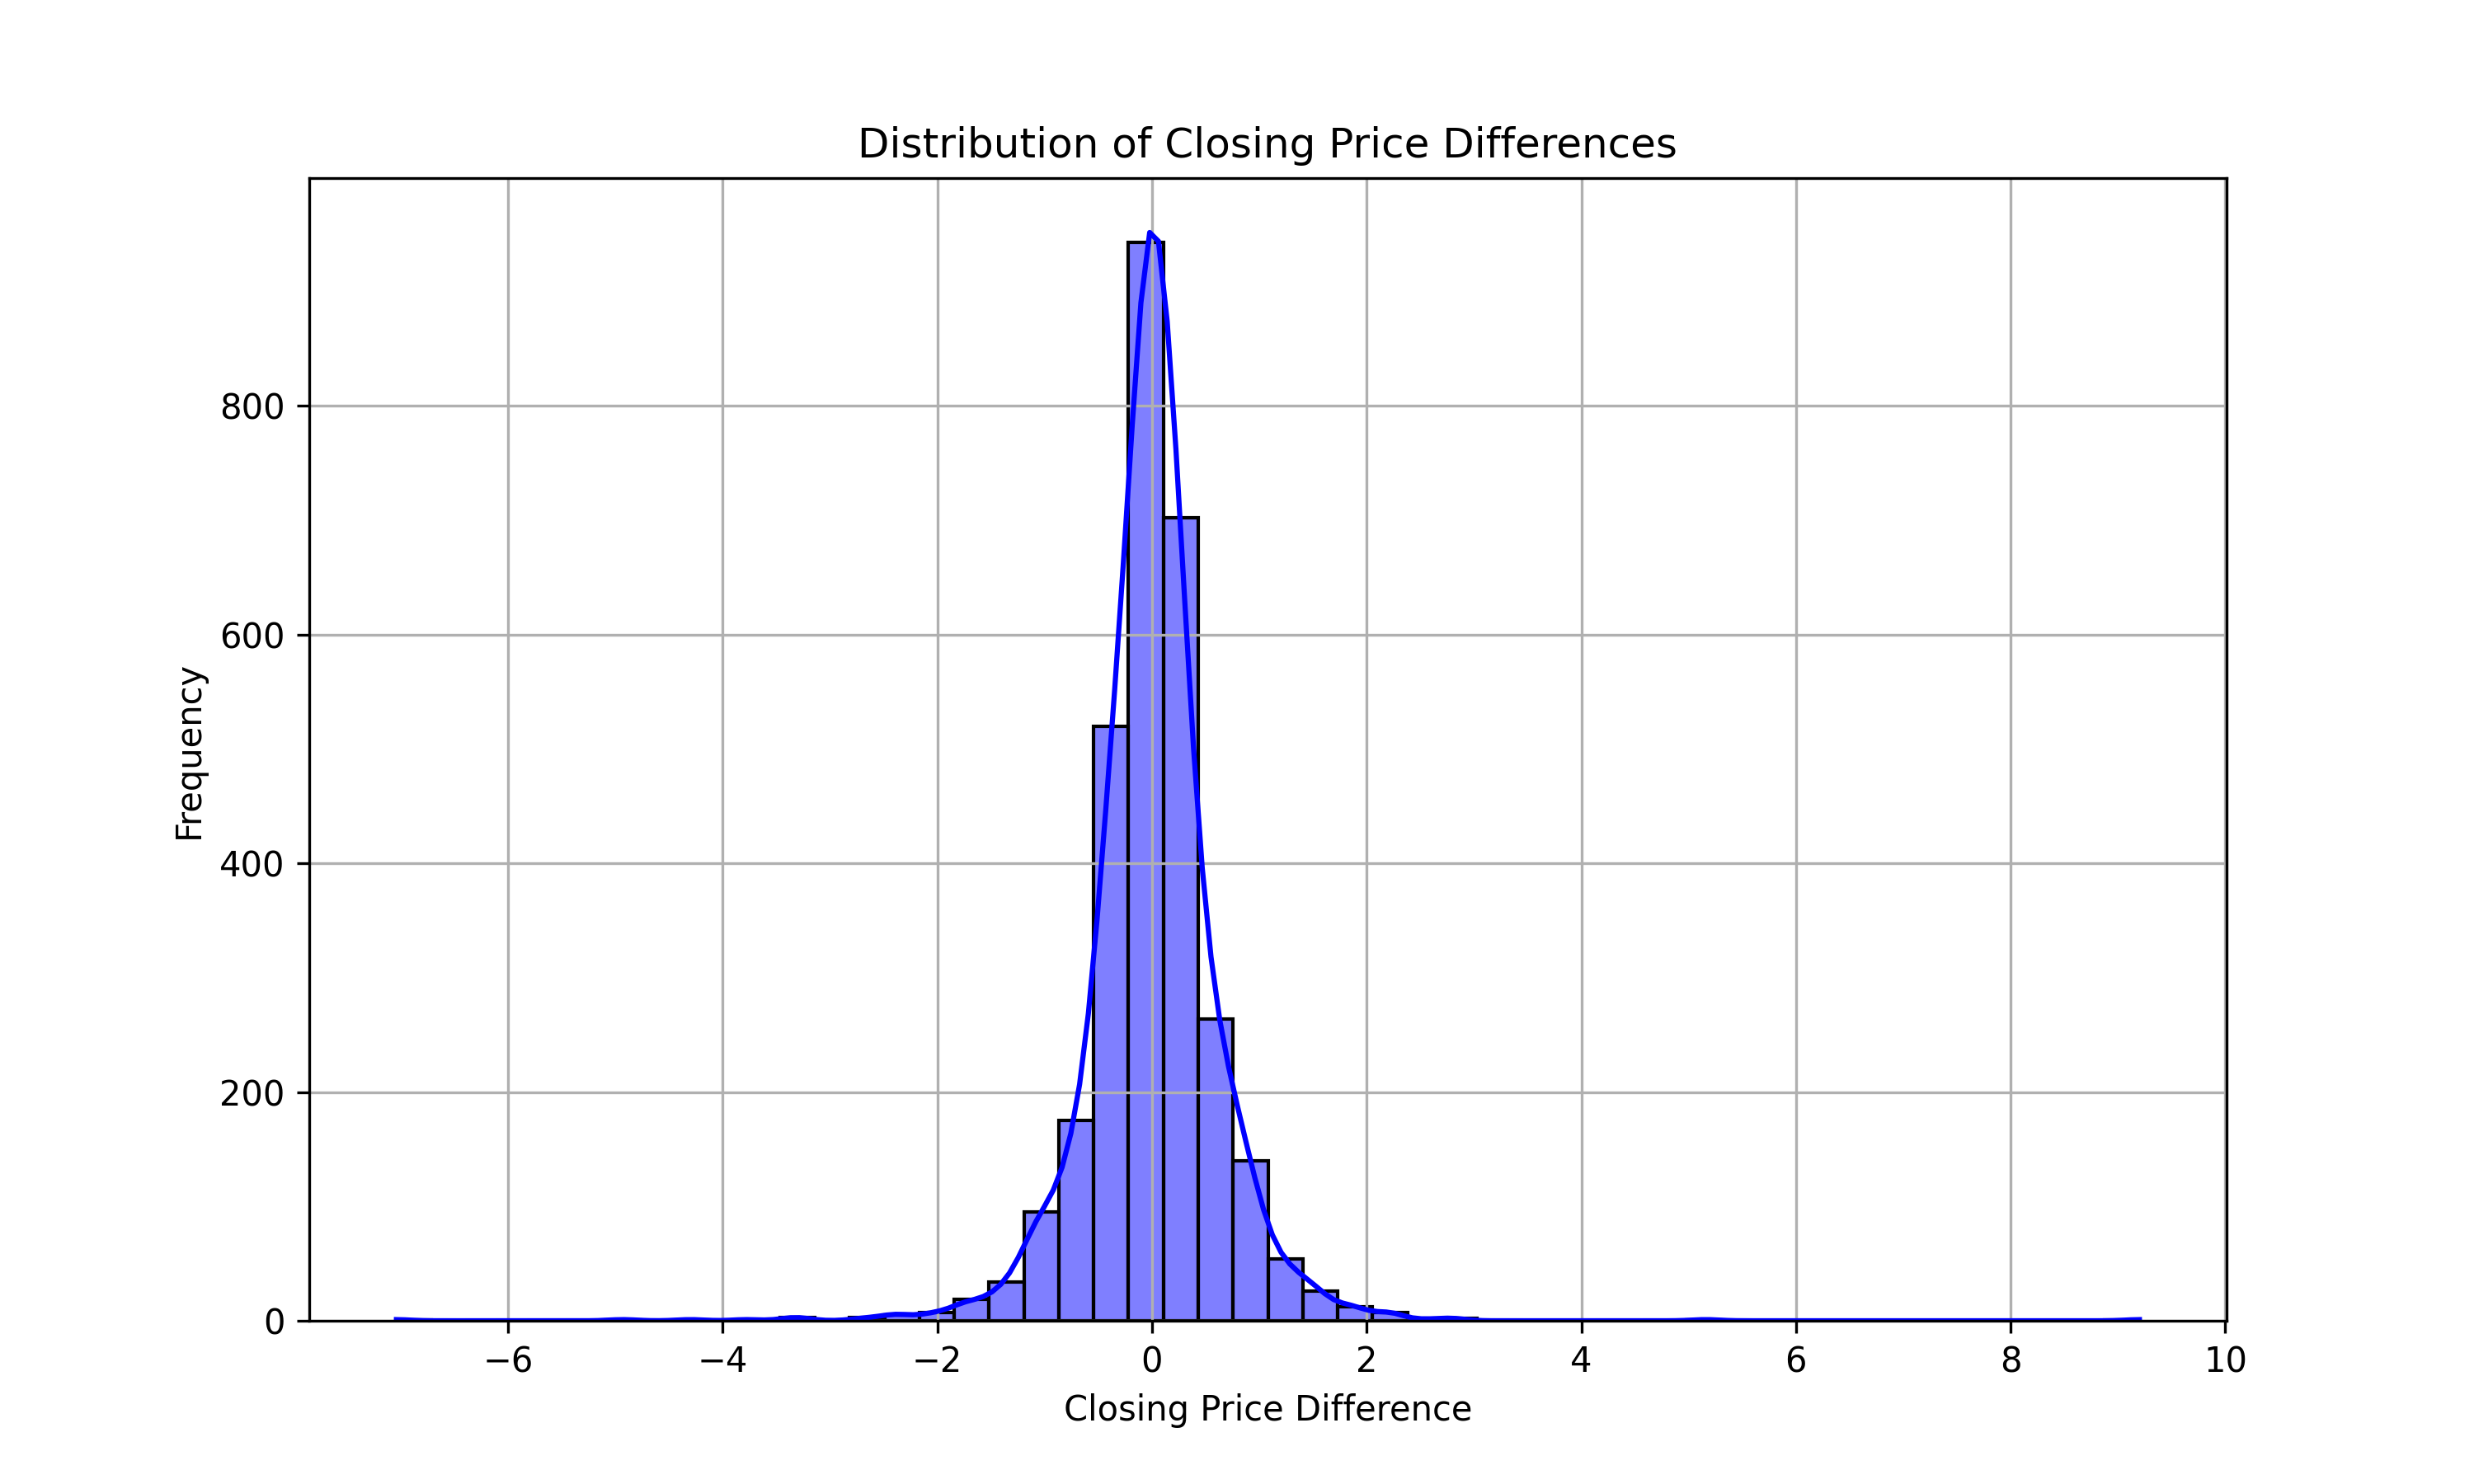
\includegraphics[width=0.8\textwidth]{distribution_closing_price_diff.png}
    \caption{Distribution of Closing Price Differences}
    \label{fig:dist}
\end{figure}

\subsection{Model Comparison}
In figure \ref{fig:comparison} a bar chart comparing all model performaces using error metrics:
\begin{itemize}
    \item \textbf{Mean squared error (mse)}:
        \begin{itemize}
        \item MSE measures the mean of actual and predicted squared diffrences value.
        \item It means a higher Mean Squared Error value  bad performance (model prediction deviates from actual values)
        \end{itemize}
    \item \textbf{r2 score (Coefficient of Determination )}:
    \begin{itemize}
    
        \item r2 score shows the model's capacity to explain data variability .
        \item A low r2 score means model performs poorly. 
    \end{itemize}
    \item \textbf{MAE}:
        \begin{itemize}

        \item MAE measures the mean diffrence of acual values and predicted values.
        \item A low MAE means model better predictive accuracy. 
        \end{itemize}
\end{itemize}

\begin{figure}[H]
    \centering
    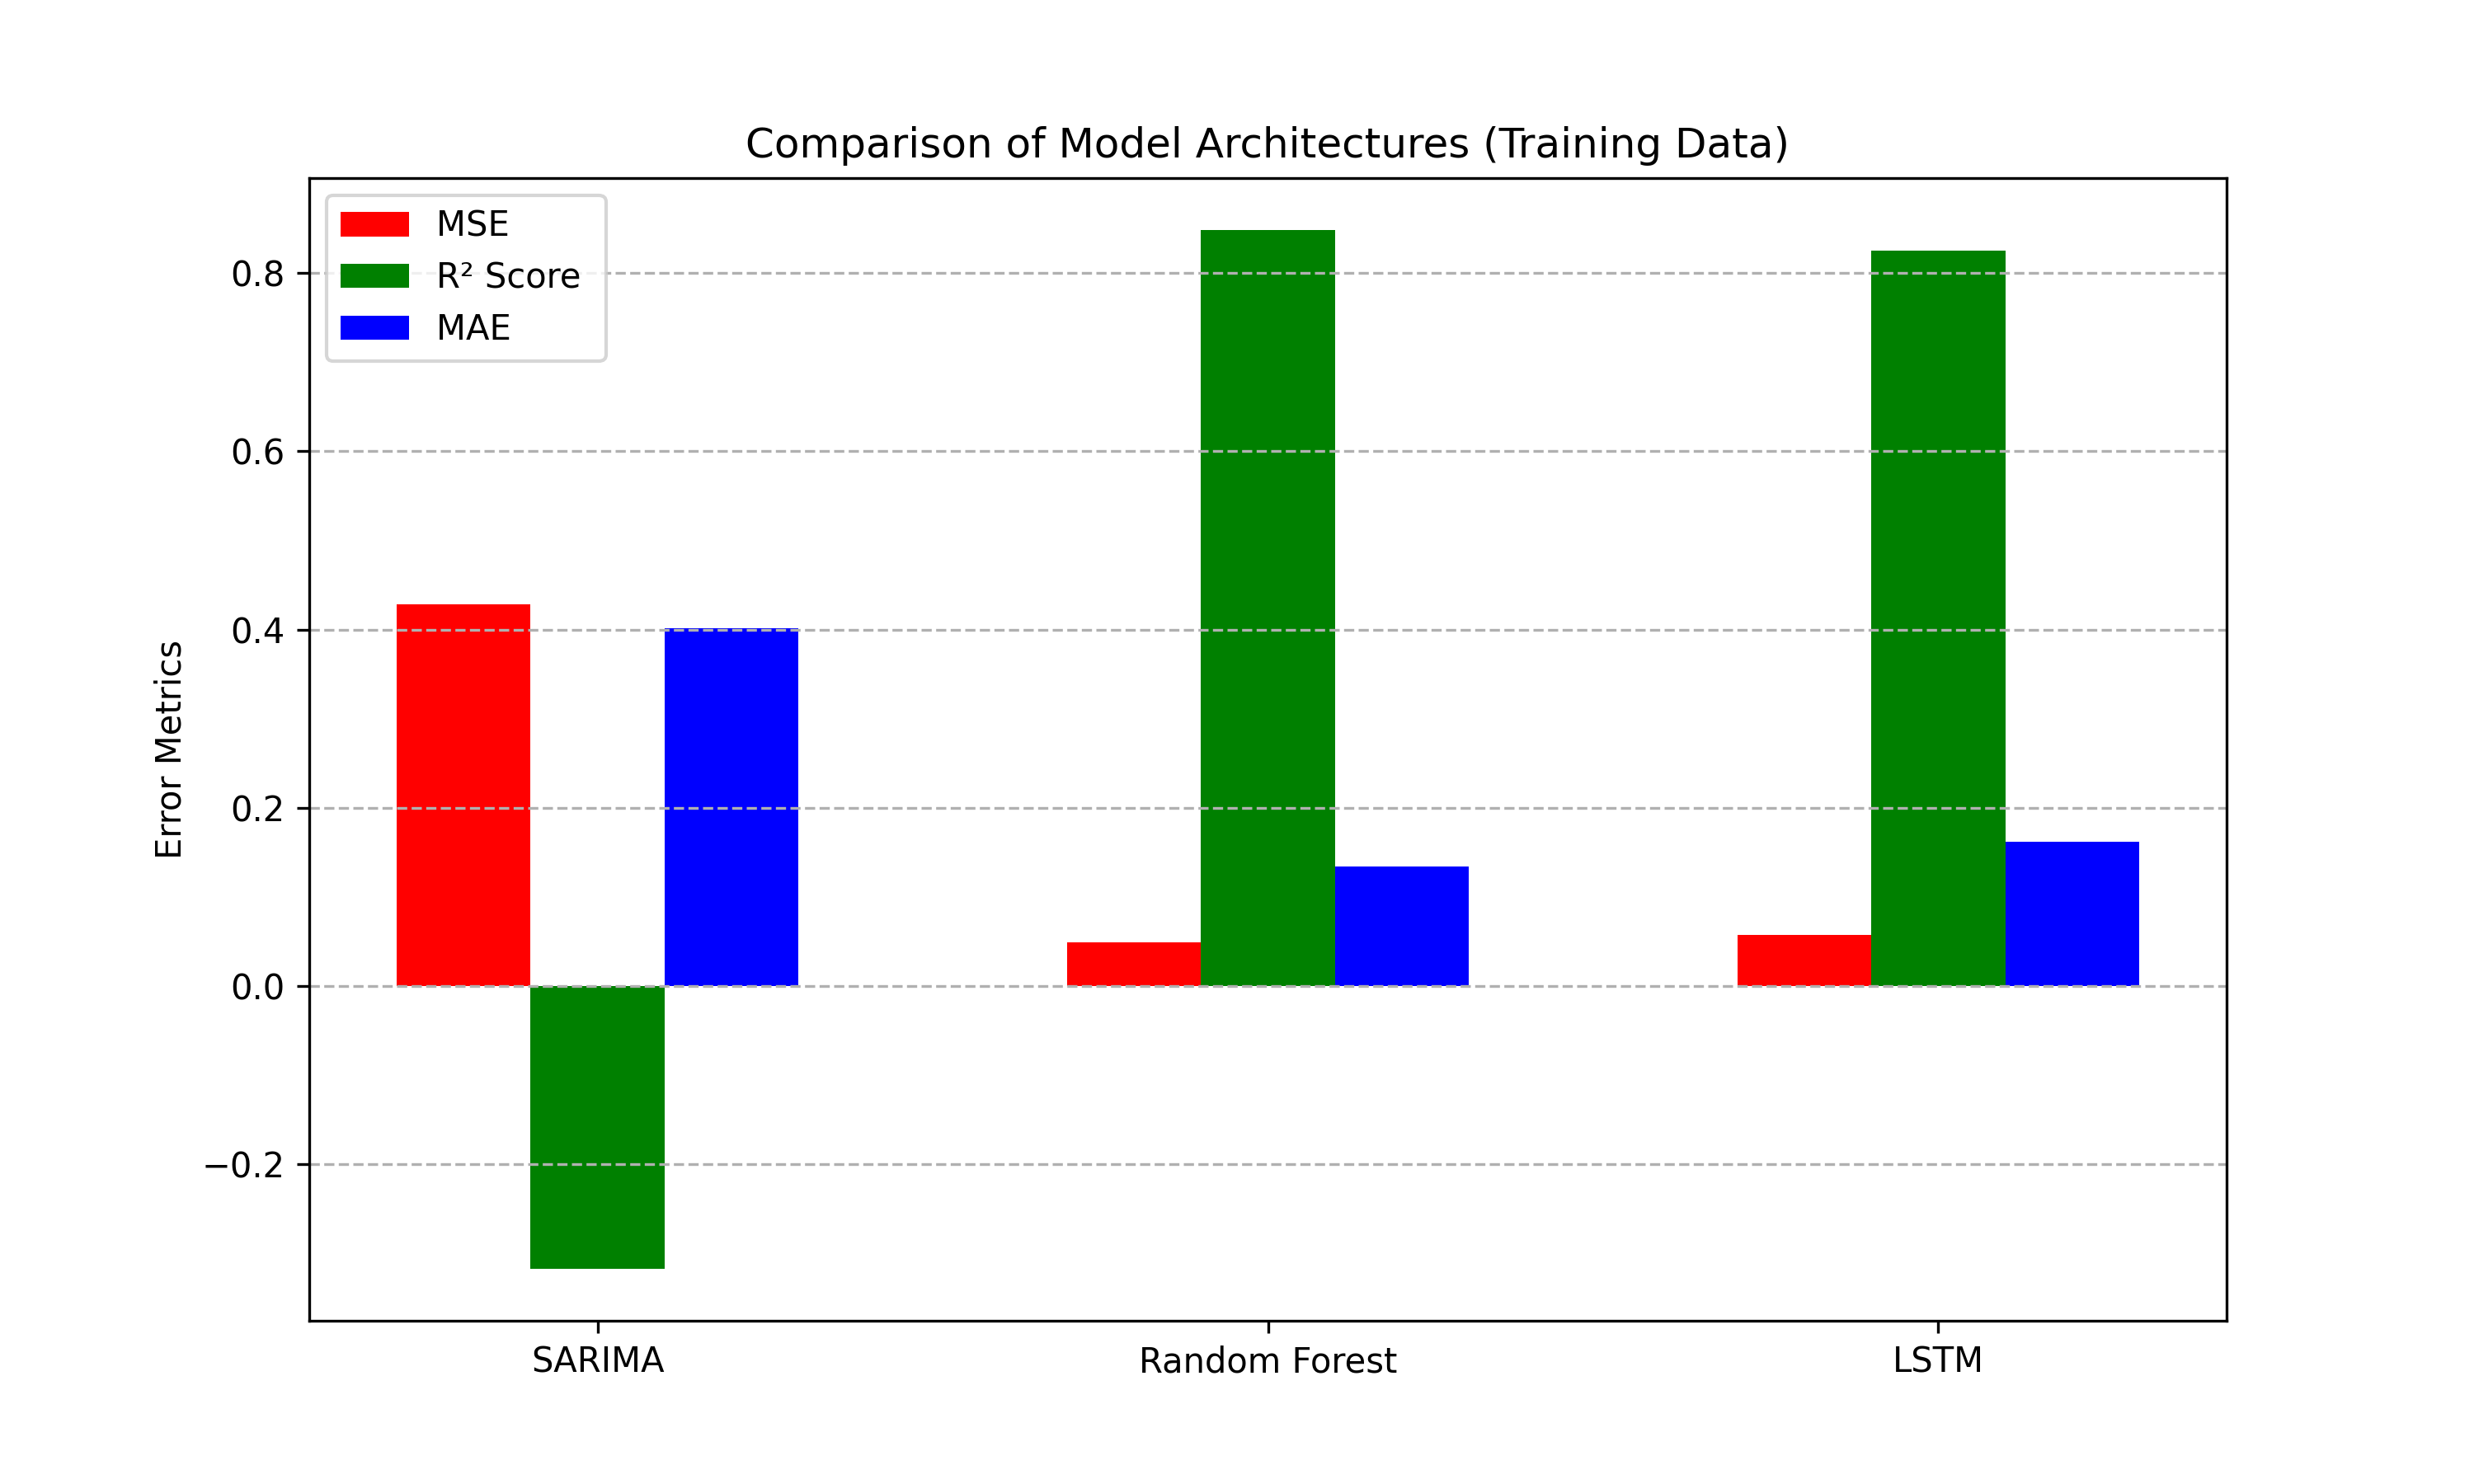
\includegraphics[width=0.8\textwidth]{model_comparison_train.png}
    \caption{Model Performance Comparison}
    \label{fig:comparison}
\end{figure}

\section{Conclusion}
Based on  data performance analysis supports the following results:\begin{itemize}
    \item \textbf{SARIMA} performs poorly, with high MSE and MAE, and a negative r2 score value, indicating bad fit to training dataset.
    \item \textbf{Random Forest and LSTM} have lower MSE and MAE values compare to \textbf{SARIMA} model and with high r2 score , indicating great performance on training dataset.
\end{itemize}

In summary, \textbf{SARIMA} does not perform well on  training dataset, while \textbf{ Random Forest and LSTM} perform well on the training dataset.
\end{document}
